\setcounter{section}{3}\setcounter{equation}{3}
% Official published.tex lines 1288–1297: Disjoint colour sets and joined-boundary notation
Let  $A_1, A_2, \ldots, A_n$ be disjoint finite sets, and $A = \sqcup_{i=1}^n A_i$
their union. The complete intersection ideal
\begin{equation*}
  C = (m(A_1), m(A_2), \ldots, m(A_n))  \sus k[A]
\end{equation*}
is the SR-ideal of the join
of the boundaries of simplices
\begin{equation} \label{eq:liaison-join}
  \Delst(\Ab) = \pd \Delta(A_1) * \pd \Delta(A_2) * \cdots * \pd \Delta(A_n),
 \end{equation}

\setcounter{subsection}{1}
% Official published.tex lines 1307–1310: Rainbow product notation
\subsection{Rainbow ideals}
Denote $\bfA = A_1 \times A_2 \times \cdots \times A_n$.
For $\bfa = (a_1, a_2, \ldots, a_n)$ in $\bfA$, denote
by $[\bfa ]$ the set $\{a_1, a_2, \ldots, a_n \}$. 

\setcounter{cdrthm}{1}
% Official published.tex lines 1333–1349: Rainbow generators and Definition 3.2
For $\bfa \in \bfA$ let $m(\bfa)$ be the monomial 
$\prod_{i = 1}^n a_i$. Thinking
of $A_i$ as a color class, we call such a monomial a {\it rainbow
monomial}.  The Alexander dual ideal $B$ of the complete intersection
$C = (m(A_1), \ldots, m(A_n))$ is generated by the complements
of the facets of $\Delst(\Ab)$, and so it is the monomial
ideal generated by all the  rainbow monomials. Letting
$(A_i)$ be the ``color ideal'' generated by the elements of $A_i$ (considered
as variables), then $B$ is the product of these color ideals:
\[ B  = (m(\bfa) \, | \, \bfa \in \bfA) = \prod_{i = 1}^n(A_i). \]

\begin{defi}
For a subset $T \sus \bfA$, denote by $I(T)$ the ideal generated
by $m(\bfa)$ for $\bfa \in T$. Such an ideal is called a {\it rainbow ideal}.
For the complement set $T^c = \bfA \backslash T$, we
usually write $L(T)$ for $I(T^c)$, the {\it complement} rainbow ideal.
\end{defi}

\setcounter{section}{5}\setcounter{subsection}{1}\setcounter{cdrthm}{0}\setcounter{equation}{6}\setcounter{figure}{5}
% Official published.tex lines 1914–1945: Product cells and saturated complex Definition 5.2
A finite set $A$ gives rise to the geometric
simplex spanned by the elements of $A$:
\[ \Delta(A) = \left\{\sum_{a \in A} \gamma_a \cdot a \, | \, 0 \leq \gamma_a \leq 1,  \sum_{a \in A} \gamma_a = 1 \right\} \sus \RR^A. \]
Given finite non-empty sets $ A_1, A_2, \ldots, A_n$, 
we get a polytope: 
\[ \Pi(\Ab) = \Delta(A_1) \times \Delta(A_2) \times \cdots
\times \Delta(A_n) \sus \times_{i = 1}^n \RR^{A_i} = \RR^A. \]
Its dual (or polar) polytope
is the join
\[ \Delst(\Ab) =  \pd \Delta(A_1) * \pd \Delta(A_2) * \cdots * \pd \Delta(A_n).
\]
The set of vertices of $\Pi(\Ab)$ is the set $A_1 \times \cdots \times
A_n$.

\begin{nota}
  When  $R_i \sus A_i$ for $ i = 1, \ldots, n$ are {\it non-empty} subsets,
  we write $\Rb \susst \Ab$.
\end{nota}


\begin{defi}
  The polytope $\Pi(\Ab)$ gives rise to a cell complex $\Cgeo(\Ab)$,
  actually a polyhedral cell complex,
whose cells are the $\Pi(\Rb)$ with $\Rb \susst \Ab$. 
The dimension of such a cell is $\sum_i |R_i| - n$.
A subset $T \sus A_1 \times A_2 \times \cdots \times A_n$
induces a cell subcomplex $C(T)$ of $\Cgeo(\Ab)$ consisting of all
$\Pi(\Rb)$ such
$R_1 \times R_2 \times \cdots \times R_n \sus T$.
We say $C(T)$ is the {\it saturated} cell sub-complex of
$\Cgeo(\Ab)$ associated to $T$. 
\end{defi}

% Official published.tex lines 1950–1961: Augmented chain complex and reduced homology
\medskip
\noindent{{\bf The (augmented) chain complex:}}
\begin{equation} \label{eq:minfree-Ct}
  \Ctbu(T): C_{-1}(T) \vpil C_0(T) \vpil C_1(T) \vpil
  \cdots \vpil C_p(T) \vpil \cdots ,
\end{equation}
where $C_p(T)$ is the $k$-vector space with basis all cells
of $\Cgeo(T)$ of dimension $p$ (and $C_{-1}(T)$ is the one-dimensional
vector space with basis the empty cell), and standard differentials
(see~\eqref{eq:minfree-diff} below). The homology groups are the
reduced homology groups. Note that $\tilde{H}_{-1}(\Ctbu(T)) \neq 0$ iff
$T$ is empty. 

% Official published.tex lines 1963–1995: Ring, monomial labels, free modules and signed differential
Let $S$ be the polynomial ring $k[A]$ whose variables
are the elements of $A = A_1 \cup \cdots \cup A_n$. 
A vertex $\bfa = (a_1,a_2, \ldots, a_n)$ of $\Pi(\Ab)$
may be labelled by the monomial
$m(\bfa) = a_1a_2\cdots a_n$. The cell $\Pi(\Rb)$ is then labelled by
the least common multiple of the monomials on its vertices. This is
simply
\[ m(\Rb) = m(R_1)m(R_2) \cdots m(R_n), \text{ where }
  m(R_i) = \prod_{r \in R_i}r,\]
which is a monomial of degree $\dim \Pi(\Rb) + n$. 

\medskip
\noindent{\bf The (augmented) free cellular complex:}
  For $T \sus A_1 \times \cdots \times A_n$, this induces a labelling
by monomials of the cell sub-complex $\Cgeo(T)$.
By~\cite[Section 4]{MiSt} it then gives a {\it free cellular complex}
\[ \Ctalg(T) : \Cal_{-1}(T) \vmto{d_0} \Cal_0(T) \vmto{d_1}
  \cdots \vpil \Cal_p(T) \vpil \cdots , \]
where
$\Cal_p(T)$ is the free $S$-modules with generators all cells $\Pi(\Rb)$ in
$\Cgeo(T)$ of dimension $p$ (and $\Cal_{-1}(T) = S$).
The image of $d_0$ is $I(T)$.
We may put a total order on each $A_i$. Together with the ordered
sequence $A_1, A_2, \ldots, A_n$, this gives a total order on the
union $A = \cup_1^n A_i$. Then $\Rb \sus^{*} \Ab$ inherits a total order on
$R = \cup_1^n R_i$. For $b \in R$ denote by $\pot(b)$ its position in
this total order. For $p \geq 1$
the differential $d^p$ is then given by
\begin{equation} \label{eq:minfree-diff}
  \Pi(\Rb) \mapsto \sum_{\begin{matrix} i = 1, \ldots, n\\
      b \in R_i, |R_i| \geq 2 \end{matrix}}  (-1)^{\pot(b)} b \cdot
  \Pi(R_1, \ldots, R_i\backslash \{b \}, \ldots, R_n).
\end{equation}

% Official published.tex lines 1997–2039: Whole Example 5.3 with native TikZ and full-box exactness
\begin{exam} Let $A_1 = \{a_1, b_1\}$ and $A_2 = \{ a_2,b_2\}$ and
  $T = A_1 \times A_2$. The product polytope $\Pi (\Ab)$ is the
  square labelled as in Figure~\ref{fig:cell-square}.

\begin{figure}[ht]
\begin{center}

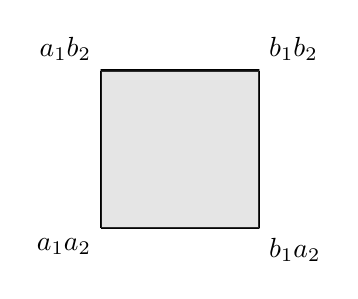
\begin{tikzpicture}[thick,scale=2]

\coordinate[label=-135:{$a_1a_2$}] (A1) at (0,0);
\coordinate[label=135:{$a_1b_2$}] (A2) at (0,1);
\coordinate[label=45:{$b_1b_2$}] (A3) at (1,1);
\coordinate[label=-45:{$b_1a_2$}] (A4) at (1,0);


\draw (A1) edge[] (A2); 
\draw (A2) edge[] (A3); 
\draw (A4) edge[swap] (A3); 
\draw (A1) edge[swap] (A4); 


\draw[fill=lightgray, opacity=0.4] (A1)--(A2)--(A3)--(A4)--(A1);

\end{tikzpicture}

\end{center}
\caption{The square $\Pi(\Ab)$, with monomial labels on vertices}
\label{fig:cell-square}
\end{figure}
  The augmented chain complex is
  \[ k \vpil k^4 \vpil k^4 \vpil k, \]
  which has no homology, it is acyclic.
  Let $S = k[a_1,b_1, a_2, b_2]$. The rainbow ideal is
  $I(T) = (a_1a_2, a_1b_2, b_1a_2, b_1b_2)$. The augmented  free cellular complex is
  \[ S \overset{d}{\vpil} S(-2)^4 \vpil S(-3)^4 \vpil S(-4). \]
  The image of $d$ is $I(T)$, and in this case,
  omitting the first term,  the complex is a minimal free resolution of $I(T)$. 
In general, if $T$ is the full $A_1 \times \cdots \times A_n$, the free cellular
complex is always a minimal free resolution of $I(T)$. Finding out for
which $T$ this free cellular
complex {\it is} a resolution, Theorem~\ref{thm:cell-linres},
is an aspect of the main result of our article. 
\end{exam}

\setcounter{fact}{0}
% Official published.tex lines 2041–2060: Linear degrees, restrictions and Fact 1
The generators of $\Cal_p(T)$ for $p \geq 0$ have degrees $p+n$,
so $\Ctcal_{\geq 0}(T)$ is a {\it linear}
free cellular complex.
The free cellular complex $\Ctalg(T)$ is $\NN^A$-graded. A family of subsets
$\Rb \susst \Ab$ gives a restriction
$T_{|R} = T \cap (R_1 \times \cdots \times R_n)$. 
It also gives a squarefree degree $\deg(\Rb) \in \NN^A$.
The free cellular complex  $\Ctalg(T)_{|\deg(\Rb)}$ in this specific degree
identifies as the augmented chain complex $\Ctbu(T_{|\Rb})$
(see~\eqref{eq:minfree-Ct}).

\begin{fact} \label{fact:cell-hom} Let $\Rb \sus^* \Ab$. 
  The homology of the augmented free cellular complex $\Ctalg(T)$
  in degree $\deg(\Rb) \in \NN^A$ is the reduced homology
  \[ H_i({\Ctalg}(T))_{\deg(\Rb)} = {H}_i(\Ctbu(T_{|\Rb})),
    \, \, i \geq -1.\]
\end{fact}

This is standard and rather immediate from the above,
see~\cite[Section 4]{MiSt}.

\setcounter{cdrthm}{3}
% Official published.tex lines 2065–2068: Proposition 5.4 homology-gap statement
\begin{prop} \label{pro:cellcx-homology}
  For $p \geq 0$, the homology group $ H_p({\Ctalg}(T))$
 can only be nonzero in degrees $\geq p+n+2$.
\end{prop}

% Official published.tex lines 2070–2102: Full Proposition 5.4 saturation proof
\begin{proof}
  In short, this is a consequence of $C(T)$ being a saturated cell complex.
 All generators of $\Cal_p(T)$ are in degree $p+n$.
  Thus $\ker d_{p}$ is generated in degrees $\geq p+n+1$.
Let $u$ be a generator of $\ker d_p$ of degree $p+n+1$.
The free cellular complex is $\NN^A$-graded, and so we may assume $u$ is
  homogeneous for this grading.
  This degree  is also squarefree
  as it is a minimal generator. Its degree is then  $\deg(\Rb)$
  for some $\Rb \susst \Ab$.
  Consider the free cellular complex $\Ctalg(\Rb)$. We have subcomplexes
  \[ \Ctalg(T_{|\Rb}) \sus \Ctalg(\Rb), \quad \Ctalg(T_{|\Rb}) \sus \Ctalg(T).\]
The latter is an isomorphism in degree $\deg(\Rb)$. 
  Thus if $\ker d_{p}$ has a generator $u$ in degree $\deg(\Rb)$, due to
  $\ker d_p^{\Ctalg(T_{|R})} \hookrightarrow \ker d_p^{\Ctalg(\Rb)}$ we get
  a generator of the latter kernel (in degree $\deg(\Rb)$),
  of total degree $p+1+n$.
  But $\ker d_p^{\Ctalg(\Rb)} = \im d_{p+1}^{\Ctalg(\Rb)}$
and $\Cal_{p+1}(\Rb)$ is the free rank one $S$-module
  $S \! \overset{}{\cdot} \! {\Pi(\Rb)}$,  with the generator $\Pi(\Rb)$ of degree $p+1+n$.
  This maps to a sum involving every face of $\Pi(\Rb)$ of dimension
  $p$. But due to the commutativity of the inclusion maps and differentials
  of 
$\Ctalg(T_{|\Rb}) \hookrightarrow \Ctalg(\Rb)$, 
 the degree $p+n$ part $\Cal_p(T_{|\Rb})$ must have
 each of the generators corresponding to a face of $\Pi(\Rb)$
 of dimension $p$. 
  In particular all vertices of $\Pi(\Rb)$ must be in $T$.  Since
  $\Cgeo(T)$ is saturated, 
  the full cell $\Pi(\Rb)$ is in $\Cgeo(T)$.
  Then the generator 
  $u$ of $\ker d_p$ is the image of a cell in $\Cal_{p+1}(T)$. 
\end{proof}

\setcounter{cdrthm}{4}
% Official published.tex lines 2110–2115: Whole counted Theorem 5.5
\begin{theo} \label{thm:cell-linres}
  Let $T \sus A_1 \times \cdots \times A_n$. If $I(T)$ has
  linear resolution, the free cellular complex  $\Ctcal_{\geq 0}(T)$ is its minimal
  free resolution. (And  $\Ctcal_{\geq 0}(T)$ is a minimal free resolution
  precisely in this case.)
\end{theo}

% Official published.tex lines 2117–2153: Full Theorem 5.5 comparison and cokernel proof with xymatrix
\begin{proof}
  Let $\Falg$ be a minimal free resolution of $I(T)$. As $I(T)$ is
  $\NN^A$-graded, the same holds for $\Falg$. Since $\Falg$ is a resolution,
  and $\Calg(T)$ consists of free modules, there is a morphism
  $\phi : \Calg(T) \pil \Falg$ lifting the identity map on $I(T)$.
  Both $\Fal_0$ and $\Cal_0(T)$ have free bases mapping bijectively to the
  minimal generators of $I(T)$, the monomials $m(\bfa)$ for $\bfa \in T$.
  So there is an isomorphism $\Fal_0 \iso \Cal_0(T)$.

  Assume $\phi_i$ is an isomorphism for $i \leq p$. Consider the diagram:
 \[ \xymatrix{ \Cal_p(T) \ar[d]^{\phi_p} &
      \Cal_{p+1}(T) \ar[l]^{d_{p+1}^{\Cal}} \ar[d]^{\phi_{p+1}} \\
      \Fal_p & \Fal_{p+1}  \ar[l]^{d_{p+1}^{\Fal}}.} \]
  Since $\phi_p$ is injective, and $d_{p+1}^{\Cal}$ is injective on
  the vector space of generators, which has degree $p+n+1$, 
  the right vertical map $\phi_{p+1}$ is also injective on
  the vector space of generators. 
    The map $\phi_{p+1}$ is then injective since
    both its domain an codomain are free with generators in degree $p+1+n$.
    
    
  Let $Q_{p+1}$ be the cokernel of the right vertical map. It is an $S$-module
  generated in degree $p+n+1$. By the long exact cohomology sequence of
  the short exact sequences of complexes
  \[ 0 \pil \Cal_{\leq p+1}(T) \pil \Fal_{\leq p+1} \pil Q_{p+1}[-p-1] \pil 0 \]
(where $[-p-1]$ denotes that $Q_{p+1}$ is in homological degree $p+1$)
  we see that $Q_{p+1}$ maps surjectively to the homology $H_p(\Calg(T))$.
  So the latter module is generated in degree $p+n+1$. But it has no
  homology in this degree, by Proposition~\ref{pro:cellcx-homology}.
 Hence this homology module vanishes.
  Then
  \[ H_{p+1}(\Fal_{\leq p+1}) \pil H_{p+1}(Q_{p+1}[-p-1]) = Q_{p+1} \]
  is surjective, where the left module is in fact the kernel
  $\ker d_{p+1}^{\Fal}$.
  Since this kernel is generated in degree $p+n+2$, this again implies
  that $Q_{p+1} = 0$. Whence $\phi_{p+1}$ is an isomorphism. 
\end{proof}

